\documentclass[a4paper,10pt]{article}

%A Few Useful Packages
\usepackage{marvosym}
\usepackage{fontspec} 					%for loading fonts
\usepackage{xunicode,xltxtra,url,parskip} 	%other packages for formatting
\RequirePackage{color,graphicx}
\usepackage[usenames,dvipsnames]{xcolor}
\usepackage[big]{layaureo} 				%better formatting of the A4 page
% an alternative to Layaureo can be ** \usepackage{fullpage} **
\usepackage{longtable} 				%for experience
\usepackage{titlesec}					%custom \section
\usepackage{amsmath}
\usepackage{amsfonts}
\usepackage[vlined,linesnumbered,ruled]{algorithm2e}

%Setup hyperref package, and colours for links
\usepackage{hyperref}
\definecolor{linkcolour}{rgb}{0,0.2,0.6}
\hypersetup{colorlinks,breaklinks,urlcolor=linkcolour, linkcolor=linkcolour}

%FONTS
\defaultfontfeatures{Mapping=tex-text}
\setmainfont[SmallCapsFont = Fontin SmallCaps]{Fontin}

%CV Sections inspired by: 
%http://stefano.italians.nl/archives/26
\titleformat{\section}{\Large\scshape\raggedright}{}{0em}{}[\titlerule]
\titlespacing{\section}{0pt}{3pt}{3pt}

%tweak page height
%\addtolength{\topmargin}{-.125in}
%\addtolength{\textheight}{0.25in}

%-------------WATERMARK TEST [**not part of a CV**]---------------
\usepackage[absolute]{textpos}

\setlength{\TPHorizModule}{30mm}
\setlength{\TPVertModule}{\TPHorizModule}
\textblockorigin{2mm}{0.65\paperheight}
\setlength{\parindent}{0pt}

\newcommand{\problem}[1]{\section*{Problem #1}}
\newcommand{\answer}{\paragraph{Answer:}}
\newcommand{\proof}{\paragraph{Proof:}}
\newcommand{\qed}{\hfill \ensuremath{\Box}}
\newcommand{\todo}{\textcolor{red}{TODO}{} }

% TODO
\newcommand{\nless}{\textcolor{red}{TODO!!!}{} }

%--------------------BEGIN DOCUMENT----------------------
\begin{document}

%WATERMARK TEST [**not part of a CV**]---------------
\font\wm=''Baskerville:color=787878'' at 8pt
\font\wmtoday=''Baskerville:color=FF1493'' at 8pt
{\wm 
	\begin{textblock}{1}(0,0)
		\rotatebox{-90}{\parbox{500mm}{
			Typeset by Yang ZHANG with \XeTeX\ on {\wmtoday \today}
		}
	}
	\end{textblock}
}

\pagestyle{empty} % non-numbered pages

\font\fb=''[cmr10]'' %for use with \LaTeX command

%--------------------TITLE-------------
\par{\centering
  {\Large Algorithms and Complexity Analysis}
  \\\vspace{0.5em}
  { Instructed by Yin ZHAO, Spring 2011, Tsinghua University}
  \\\vspace{1.5em}
	{\Huge Solutions for homework 3\vspace{1em}
	}\bigskip\par}

%--------------------SECTIONS-----------------------------------

\problem{6.3-2}
Why do we want the loop index $i$ in line 2 of \textsc{Build-Max-Heap} to decrease from 
$\left\lfloor \frac{length[A]}{2}\right\rfloor$ to 1 rather than increase from 1
to $\left\lfloor \frac{length[A]}{2}\right\rfloor$?

\begin{algorithm}[H]
\caption{\textsc{Build-Max-Heap}$(A)$}
$heap$-$size[A]\leftarrow length[A]$\\
\For{$i \leftarrow \left\lfloor\frac{length[A]}{2}\right\rfloor$ \textnormal{\textbf{downto}} $1$} {
  \textsc{Max-Heapify}$(A, i)$
}
\end{algorithm}

\answer

This is because we must make sure that the smaller subtrees are changed to heaps first, so that the
algorithm could build bigger subtrees correctly. If we increase the index $i$ from 1 to
$\left\lfloor\frac{length[A]}{2}\right\rfloor$, the heap property cannot be correctly preserved.\\

For example, consider the input array $\langle 3, 1, 2, 4\rangle$. The correct algorithm will
runs like this,

\begin{center}
  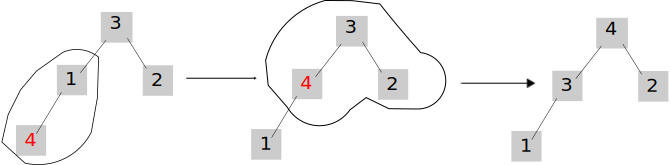
\includegraphics[width=300pt]{sol3-fig1.pdf}
\end{center}

while \textbf{Algorithm 1} runs like this,

\begin{center}
  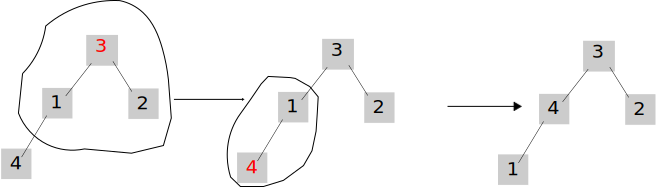
\includegraphics[width=300pt]{sol3-fig2.pdf}
\end{center}

and the result is obviously not a max heap.

\qed

\problem{7-1 Hoare partition correctness}
The version of \textsc{Partition} given in this chapter is not the original partitioning algorithm. 
Here is the original parition algorithm, which is due to T.Hoare:

\begin{algorithm}[H]
\caption{\textsc{Hoare-Partition}$(A, p, r)$}
$x \leftarrow A[p]$\\
$i \leftarrow p - 1$\\
$j \leftarrow r + 1$\\
\While{$true$}{
  \Repeat{$A[j] \leq x$}{
    $j \leftarrow j - 1$\\
  }
  \Repeat{$A[i] \geq x$}{
    $i \leftarrow i + 1$\\
  }
  \If{$i < j$}{
    exchange $A[i] \leftrightarrow A[j]$
  }\Else{
    \Return $j$
  }
}
\end{algorithm}

\begin{description}
\item[a. \hspace{9pt}] Demonstrate the operation of \textsc{Hoare-Partition} on the array 
$A=\langle13, 19, 9, 5, 12, 8, 7, 4,\\ 11, 2, 6, 21\rangle$, showing the values of
the array and auxiliary values after each iteration of the \textbf{while} loop in lines 4\textasciitilde 11.\\

\end{description}
The next three questions ask you to give a careful argument that the procedure \textsc{Hoare-Partition} is correct.
Prove the following:

\begin{description}
\item[b. \hspace{9pt}] The indices $i$ and $j$ are such that we never access an element of $A$ outside
the subarray $A[p\ldots r]$.

\item[c. \hspace{9pt}] When \textsc{Hoare-Partition} terminates, it returns a value $j$ such that $p\leq j < r$.

\item[d. \hspace{9pt}] Every element of $A[p\ldots j]$ is less than or equal to every element of
$A[j + 1\ldots r]$ when \textsc{Hoare-Partition} terminates.
\end{description}

The \textsc{Partition} procedure shown below separates the pivot value (originally in $A[r]$) from the
two partitions it forms. The \textsc{Hoare-Partition} procedure,
on the other hand, always places the pivot value (originally in $A[p]$) into one of the two paritions
$A[p\ldots j]$ and $A[j + 1\ldots r]$. Since $p\leq j < r$, this
split is always nontrivial.

\begin{algorithm}[H]
\caption{\textsc{Partition}(A, p, r)}
$x\leftarrow A[r]$\\
$i \leftarrow p - 1$\\
\For{$j \leftarrow p$ \KwTo $r-1$}{
  \If{$A[j] \leq x$} {
    $i \leftarrow i + 1$\\
    exchange $A[i] \leftrightarrow A[j]$\\
  }
}
exchange $A[i + 1]\leftrightarrow A[r]$\\
\Return {$i + 1$}
\end{algorithm}

\begin{description}
\item[e. \hspace{9pt}] Rewrite the \textsc{Quicksort} procedure to use \textsc{Hoare-Partition}.
\end{description}

\newpage

\answer

\begin{description}
\item[a. \hspace{9pt}] The iteration is shown in the following table:

\begin{center}
\begin{tabular}{|c|c|c|c|}
\hline
Loop No. & $A$ & $i$ & $j$\\\hline
1 & $\langle 6, 19, 9, 5, 12, 8, 7, 4, 11, 2, 13, 21\rangle$ & 1 & 11\\\hline
2 & $\langle 6, 2, 9, 5, 12, 8, 7, 4, 11, 19, 13, 21\rangle$ & 2 & 10\\\hline
3 & $\langle 6, 2, 9, 5, 12, 8, 7, 4, 11, 19, 13, 21\rangle$ & 10 & 9\\\hline
\end{tabular}
\end{center}

\item[b. \hspace{9pt}] First of all, $j$ was given initial value $r + 1$, and it is decreased before
the access of $A[j]$, so $j\leq r$ when $j$ is used as an index to $A$.
Similarly we have $i \geq p$.

Suppose that when the procedure \textbf{return}s, there is a $k$ such that $j < k < i$.
Since the \textbf{repeat} statement of lines 5\textasciitilde  7 halts only when $A[j] \leq x$, 
we know that $A[k] > x$. Similarly, the \textbf{repeat} statement of lines 8\textasciitilde 10
halts only when $A[j] \geq x$, which requires $A[k] < x$. From this contradiction we knows
that the $k$ does not exist, which means $j \geq i - 1$.

On each round of the \textbf{while} loop, line 6 and line 9 are both executed at least once.
If the \textbf{while} loop is executed more than once, we have $j \leq r - 1$ and
$i \geq p + 1$. With the fact that $j \geq i -1$, it is trivial to prove that 
$p \leq i \leq r$ and $p \leq j \leq r$.


Now we consider the case when the \textbf{while} loop is executed only once. The
\textbf{repeat} statement of lines 5\textasciitilde 7 halts when $A[j] \leq x$. With the fact that $A[p] = x$,
we have $j \geq p$. And the \textbf{repeat} statement of lines 8\textasciitilde 10 will halt with $i = p$.
Now we have proved that under all cases, $p \leq i \leq r$ and $p \leq j \leq r$, 
so we never access an element of $A$ outside $A[p\ldots r]$.


\item[c. \hspace{9pt}] The original question should add another requirement that $p < r$. We have
already proved that $p \leq j \leq r$. Suppose the procedure returned $j = r$, then
we know that the \textbf{while} loop is executed only once (in each \textbf{while} loop, $j$ is
decreased at least by 1). And we know that on the first round of the \textbf{while}
loop, the \textbf{repeat} statement of lines 8\textasciitilde 10 will halt with $i = p$. The \textbf{return}
statement will be reached only when $i \geq j$, that is, $p \geq r $. Now we have
a contradiction here, which means $j \neq r$, so the procedure returns $p \leq j < r$.

\item[d. \hspace{9pt}] We prove the invariant that ``after line 10, every element in $A[p \ldots i - 1]$
is less than or equal to $x$, and every element in $A[j + 1 \ldots r]$ is greater than
or equal to $x$''.

Before the first round of the \textbf{while} loop, this invariant is true, since there is no element in the
subarrays. Suppose the invariant is true before the $k$th round, then in the $k$th
round, the \textbf{repeat} statement in lines 5\textasciitilde 7 decrease $j$ until $A[j] \leq x$, so it is still
true that any element in $A[j + 1 \ldots r]$ is greater than or equal to $x$.
Similarly we know that any element in $A[p \ldots i - 1]$ is less than or equal to $x$. Lines 11\textasciitilde 14
 does not change the value of $i$ and $j$, so $i$ and $j$ remains unchanged until
the $(k + 1)$th loop. By mathematical induction we know that the invariant is true.

The procedure returns only when $i \geq j$, and we have proved $j \geq i - 1$ in question (c), so we
have either $i = j$ or $i = j + 1$. If $i = j$, since $A[i] \geq x$ and $A[j] \leq x$, 
we have $A[i] = A[j] = x$, so every element in $A[p \ldots j]$ is less than or equal to $x$,
and every element in $A[j + 1 \ldots r]$ is greater than or equal to $x$. If $i = j + 1$,
we have the same conclusion. Thus the statement of question (d) is proved.

\newpage

\item[e. \hspace{9pt}] The algoritm is given below.

\end{description}
\begin{algorithm}[H]
\caption{\textsc{Hoare-Quicksort}$(A, p, r)$}
\If{$p \leq r$}{
  \Return
}\Else{
  $j \leftarrow$\textsc{Hoare-Partition}$(A, p, r)$\\
  \textsc{Hoare-Quicksort}$(A, p, j)$\\
  \textsc{Hoare-Quicksort}$(A, j + 1, r)$
}
\end{algorithm}
\qed


\problem{7-4 Stack depth for quicksort}
The \textsc{Quicksort} algorithm of Section 7.1 contains two recursive calls to itself.
After the call to \textsc{Partition}, the left subarray is recursively sorted and then the right subarray
is recursively sorted. The second recursive call in \textsc{Quicksort} is not really necessary; it can be
avoided by using an iterative control structure. This technique, called \emph{tail recursion},
is provided automatically by good compilers. Consider the following version of quicksort, which simulates tail recursion.

\begin{algorithm}[H]
  \caption{\textsc{Quicksort'$(A, p, r)$}}
  \While {$p<r$}{
    $q\leftarrow $\textsc{Partition}$(A, p, r)$\\
    \textsc{Quicksort'}$(A, p, q-1)$\\
    $p\leftarrow q+1$\\
  }
\end{algorithm}

\begin{description}
\item[a. \hspace{9pt}] Argue that \textsc{Quicksort'}$(A, 1, length[A])$ correctly sorts the array A.

Compilers usually execute recursive procedures by using a \emph{stack} that contains pertinent information, including
the parameter values, for each recursive call. The information for the most recent call is at the top of the stack,
and the information for the initial call is at the bottom. When a procedure is invoked, its information is \emph{pushed}
 onto the stack; when it terminates, its information is \emph{popped}. Since we assume that array parameters are
 represented by pointers, the information for each procedure call on the stack requires $O(1)$ stack space.
 The \emph{stack depth} is the maximum amount of stack space used at any time during a computation.

\item[b. \hspace{9pt}] Describe a scenario in which the stack depth of \textsc{Quicksort'} is $\Omega(n)$ on an 
$n$-element input array.

\item[c. \hspace{9pt}] Modify the code for \textsc{Quicksort'} so that the worst-case stack depth is $\Omega(\lg n)$.
Maintain the $O(n\lg n)$ expected running time of the algorithm.

\end{description}

\answer

\begin{description}
  
\item[a. \hspace{9pt}] \textsc{Quicksort'} does exactly what \textsc{Quicksort} does; hence it sorts correctly.


\textsc{Quicksort} and \textsc{Quicksort'} do the same partitioning, and then each calls itself with arguments
$A, p, q − 1$. \textsc{Quicksort} then calls itself again, with arguments $A, q + 1, r$. \textsc{Quicksort'} instead
sets $p \leftarrow q + 1$ and performs another iteration of its while loop. This executes the same operations as
calling itself with $A, q + 1, r$, because in both cases, the first and third arguments ($A$ and $r$) have the same
values as before, and $p$ has the old value of $q + 1$.


\item[b. \hspace{9pt}] The stack depth of \textsc{Quicksort'} will be $\Theta(n)$ on an $n$-element input array if
there are $\Theta(n)$ recursive calls to \textsc{Quicksort'}. This happens if every call to \textsc{Partition}$(A, p, r)$
returns $q=r$. The sequence of recursive calls in this scenario is 

\textsc{Quicksort'}$(A, 1, n)$, \\
\textsc{Quicksort'}$(A, 1, n - 1)$, \\
\textsc{Quicksort'}$(A, 1, n -2 )$, \\
  $\vdots$\\
\textsc{Quicksort'}$(A, 1, 1)$.

Any array that is already sorted in increasing order will cause \textsc{Quicksort} to behave this way.


\item[c. \hspace{9pt}] The problem demonstrated by the scenario in part (b) is that each invocation
of \textsc{Quicksort'} calls \textsc{Quicksort'} again with almost the same range. To avoid such behavior,
we must change \textsc{Quicksort'} so that the recursive call is on a smaller interval of the array.
The following variation of \textsc{Quicksort'} checks which of the two subarrays returned from \textsc{Partition}
 is smaller and recurses on the smaller subarray, which is at most half the size of the current array.
 Since the array size is reduced by at least half on each recursive call, the number of recursive calls,
 and hence the stack depth, is $\Theta(\lg n)$ in the worst case. Note that this method works no matter how
 partitioning is performed (as long as the \textsc{Partition} procedure has the same functionality as the procedure
 given in Section 7.1).
 
 \begin{algorithm}[H]
 \caption{\textsc{Quicksort''}$(A, p, k)$}
 \While{$p < r$}{
  $q \leftarrow$ \textsc{Partition}$(A, p, r)$\\
  \If{$q - p < r - q$}{
    \textsc{Quicksort''}(A, p, q - 1)\\
    $p \leftarrow q + 1$\\
  }\Else{
  \textsc{Quicksort''}(A, q + 1, r)\\
  $r \leftarrow q + 1$\\
  }
 }
 \end{algorithm}
 
 The expected running time is not affected, because exactly the same work is done as before:
 the same partitions are produced, and the same subarrays are sorted.

\end{description}

\qed

\problem{8.2-4}
Describe an algorithm that, given $n$ intergers in the range 0 to $k$, preprocesses its input and then answers
any query about how many of the $n$ integers fall into a range
$[a\ldots b]$ in $O(1)$ time. Your algorithm should use $\Theta(n + k)$ preprocessing time.
\answer

The algorithm is given below. The \textsc{Preprocess} returns an array, which will be used by \textsc{Count-Interval}.

\begin{algorithm}[H]
\caption{\textsc{Preprocess}$(A, n, k)$}
Create array $C$ with size $k + 1$, index starts at $0$\\
\For{$i = 0$ to $k$}{
  $C[i] \leftarrow 0$
}
\For{$i = 1$ to $n$}{
  $C[A[i]] \leftarrow C[A[i]] + 1$
}
\tcp{Now $C[j]$ contains number of elements with value $j$}
\For{$i = 1$ to $k$}{
  $C[A[i]] \leftarrow C[A[i]] + C[A[i - 1]]$
}
\tcp{Now $C[j]$ contains number of elements in the range $[0, j]$}
\Return $C$
\end{algorithm}

\begin{algorithm}[H]
\caption{\textsc{Count-Interval}$(C, a, b)$}
\tcp{Array $C$ is returned by \textsc{Preprocess}$(A, n)$}
\If{$a \neq 0$}{
  \Return $C[b] - C[a - 1]$
}\Else{
  \Return $C[b]$
}
\end{algorithm}
\qed



\problem{8-6 Lower bound on merging sorted lists}

The problem of merging two sorted lists aries frequently. It is used as a subroutine of \textsc{Merge-Sort},
and the procedure to merge two sorted lsits is given as \textsc{Merge} in Section 2.3.1. In this problem,
we will show that there is a lower bound of $2n-1$ on the worst-case number of comparisons required to 
merge two sorted lists, each containing $n$ items.

First we will show a lower bound of $2n-o(n)$ comparisons by using a decision tree.

\begin{description}
\item[a. \hspace{9pt}] Show that, given $2n$ numbers, there are ${2n}\choose{n}$ possible ways to divide them into
two sorted lists, each with $n$ numbers.

\item[b. \hspace{9pt}] Using a decision tree, show that any algorithm that correctly merges two sorted lists uses at
least $2n-o(n)$ comparisons.

\item[c. \hspace{9pt}]  Show that if two elements are consecutive in the sorted order and from opposite lists,
then they must be compared.

\item[d. \hspace{9pt}] Use your answer to the previous part to show a lower bound of $2n-1$ comparisons for merging
two sorted lists.

\end{description}

\answer

\begin{description}
\item[a. \hspace{9pt}] There are $2n \choose n$ ways to divide $2n$ numbers into two groups. When all the elements in a group
is chosen, the sorted arrays will be defined, too. So there are exactly $2n \choose n$ ways in total.

\item[b. \hspace{9pt}] The minimum worst case decision tree height is:
\begin{eqnarray*}
\lg{2n \choose n} &=&\lg\left(\frac{(2n)!}{n!\times n!}\right) \\
    &=&\lg\left((2n)!\right) - 2\lg\left(n!\right) \\
    &=& \lg\left(\sqrt{2\pi\cdot 2n}\left(\frac{2n}{e}\right)^{2n}\left(1 +O\left(\frac{1}{2n}\right)\right)\right) 
        - 2\lg\left(\sqrt{2\pi n}\left(\frac{n}{e}\right)^{n}\left(1 +O\left(\frac{1}{n}\right)\right)\right)\\
    &=& \frac{1}{2}\lg{n} + 2n\lg\left(\frac{2n}{e}\right) 
        - 2\left(   \frac{1}{2}\lg{n} + n\lg\left(\frac{n}{e}\right)   \right) + O(1)\\
    &=& 2n - \frac{1}{2}\lg{n} + O(1)\\
    &=& 2n - o(n)
\end{eqnarray*}

\item[c. \hspace{9pt}]  We prove this by contradiction. Suppose we have array $A=(a_1 < a_2 < \cdots < a_m)$ and 
$B=(b_1 < b_2 < \cdots < b_n)$. Let $a_i$ and $b_j$ be consecutive in sorted list, and they have not been compared.
Then by merging $A'=(a_1 < \cdots < a_{i-1} < b_j < a_{i+1} <\cdots <  a_m)$ and
$B' = (b_1 < \cdots < b_{j-1} < a_i < a_{j+1}  < \cdots < b_n)$ we will have a different sorted list from same elements, 
which is a contradiction.

\item[d. \hspace{9pt}]  The following input needs exactly $2n-1$ comparisons:

$$a_1 < b_1 < a_2 < b_2 < \cdots < a_{i} < b{i} < a_{i+1} < \cdots < a_n < b_n.$$

There are $2n-1$ consecutive pairs, and they are from different lists.

\end{description}

\qed



\problem{9.3-1}
In the algorithm \textsc{Select}, the input elements are divided into groups of 5.
Will the algorithm work in linear time if they are divided into groups of 7? Argue that
\textsc{Select} does not run in linear time if groups of 3 are used.
\answer

By similar analyze, we know that the smaller part has at least

$$ 4\left(\left\lceil\frac{1}{2}\left\lceil\frac{n}{7}\right\rceil\right\rceil-2\right)\geq \frac{2n}{7} - 8.$$

So, in worst case, \textsc{Select} is recursively running on $\frac{5n}{7} + 8$ elements. Now we obtain the recurrence:

\begin{equation*}
T(n) \leq \left\{
  \begin{array}{ll}
    \Theta(1)     & \text{if $n \leq 140$,}\\
    T\left(\left\lceil\frac{n}{7}\right\rceil\right) + T\left(\frac{5n}{7} + 8\right) + O(n) & \text{if $n > 140$.}
  \end{array}
\right.
\end{equation*}

By substitution we have:

\begin{eqnarray*}
T(n)  &\leq& c\left\lceil\frac{n}{7}\right\rceil + c\left(\frac{5n}{7} + 8\right) + bn\\
&\leq& c\times\left(\frac{n}{7}+1\right) + \frac{5cn}{7} + 8c + bn\\
&=&cn + \left(9 c + bn - \frac{cn}{7}\right)
\end{eqnarray*}

Now we only need $9 c + \left(b - \frac{c}{7}\right)n \leq 0$, which could be satisfied by choosing $c > \frac{980}{77}b$.

For groups of 3, however, the algorithm no longer works in linear time.
The number of elements greater than $x$, and the number of elements less than $x$, is at least

$$2\left(\left\lceil\frac{1}{2}\left\lceil\frac{n}{3}\right\rceil\right\rceil - 2\right) \geq \frac{n}{3}-4,$$

and the recurrence becomes

$$T(n)\leq T\left(\left\lceil\frac{n}{3}\right\rceil\right)+T\left(\frac{2n}{3} + 4\right) + O(n),$$

which does not have a linear solution.

We can prove that the worst-case time for groups of 3 is $\Omega(n\lg n).$
We do so by deriving a recurrence for a particular case that takes $\Omega(n\lg n)$ times.

In counting up the number of elements greater than $x$ (and similarly, the number less than $x$), consider
the particular case in which the ``leftover'' group does contribute 2 elements greater than $x$. Then the
number of elements greater than $x$ is exactly
$$2\left(\left\lceil\frac{1}{2}\left\lceil\frac{n}{3}\right\rceil\right\rceil-1\right) + 1 
= \left\lceil\frac{n}{6}\right\rceil -1$$ 

(the $-1$ discounts $x$'s group, as usual, ant the $+1$ is contributed by $x$'s group), 
and the recursive step for elements $\leq x$ has

$$n -\left(\left\lceil\frac{n}{6}\right\rceil  -1\right) \geq n - \left(2\left(\frac{n}{6} + 1\right) - 1\right)
= \frac{2n}{3} - 1$$

 elements. Observe also that the $O(n)$ term in the recurrence is really $\Theta(n)$,
since the partitioning in step 4 takes $\Theta(n)$ (not just $O(n)$) time. Thus, we get the recurrence


$$T(n)\geq T\left(\left\lceil \frac{n}{3}  \right\rceil\right) + T\left(\frac{2n}{3} - 1\right) + \Theta(n)
\geq T\left(\frac{n}{3}\right) + T\left(\frac{2n}{3} - 1\right) + \Theta(n),$$


from which you can show that $T(n) \geq cn \log n$ by substitution. You can also see that $T(n)$ is 
nonlinear by noticing that each level of the recursion tree sums to $n$.

\qed
\end{document}


